\documentclass[11pt]{beamer}
\usetheme{Marburg}

%-------------------adding IIT logo starts-------------------

\addtobeamertemplate{sidebar right}{}{
 \vspace{-26ex}
  
\includegraphics[width = 0.2\textwidth]{Figs/iit_high_res.png}
}
%-------------------adding IIT logo ends-------------------

\usepackage[utf8]{inputenc}
\usepackage[english]{babel}
\usepackage[T1]{fontenc}
\usepackage{amsmath}
\usepackage{amsfonts}
\usepackage{amssymb}
\usepackage{graphicx}
\usepackage{subfigure}
\usepackage{comment}
\usepackage{listings}
\usepackage{xcolor}

\hypersetup{
    colorlinks=true,
    linkcolor=blue,
    filecolor=magenta,      
    urlcolor=blue,}
%    Inline Python
\definecolor{codegreen}{rgb}{0,0.6,0}
\definecolor{codegray}{rgb}{0.5,0.5,0.5}
\definecolor{codepurple}{rgb}{0.58,0,0.82}
\definecolor{backcolour}{rgb}{1,1,1}
\lstdefinestyle{mystyle}{
    backgroundcolor=\color{backcolour},   
    commentstyle=\color{codegreen},
    keywordstyle=\color{blue},
    numberstyle=\tiny\color{codegray},
    stringstyle=\color{codepurple},
    basicstyle=\ttfamily\footnotesize,
    breakatwhitespace=false,         
    breaklines=true,                 
    captionpos=b,                    
    keepspaces=true,                 
    numbers=left,                    
    numbersep=5pt,                  
    showspaces=false,                
    showstringspaces=false,
    showtabs=false,                  
    tabsize=2}
\lstset{style=mystyle}


\title[QMCPy]{QMCPy\\
    Quasi-Monte Carlo Community Software\\
    Python 3}
\author[]{Aleksei Sorokin\\
Sou-Cheng T. Choi, Fred J. Hickernell, Lynn Matar,\\
Mike McCourt}
\institute{Illinois Institute of Technology\\
    Department of Applied Mathematics\\
    Computational Math Seminar} 
\date{November 15, 2019} 

\newcommand{\dif}{\textup{d}}

\begin{document}
\begin{frame}[noframenumbering] \titlepage \end{frame}

% Add page number to footer
\addtobeamertemplate{navigation symbols}{}{%
    \usebeamerfont{footline}%
    \usebeamercolor[fg]{footline}%
    \hspace{1em}%
    \insertframenumber/\inserttotalframenumber
}


% OVERVIEW
%%%%%%%%%%%%%%%%%%%%%%%%%%%%%%%%%%%%%%%%%%
\section{Development}
    
\begin{frame}{Original \& Convenient Forms}
    \begin{equation*}
        \mu = \int_{T} g(t) \, \lambda(\dif t) = \int_{X} f(x)\rho(x) \, \dif x = \int_{X} f(x) \, \nu( \dif x)
        \label{eq:ogProblem}
    \end{equation*}
    $ g:T \rightarrow \mathbb{R}$ = original integrand \\
    $ \lambda$ = original measure\\
    $\phi: X \rightarrow T$ = change of variables\\
    $f: X \rightarrow \mathbb{R} $ = integrand after change of variables\\
    $\nu$ = well understood probability measure
\end{frame}

\begin{frame}{(Quasi-)Monte Carlo Approximation}
    \begin{equation*}
        \hat{\mu}_n = a_n \sum_{i=1}^{n} f(x_i)w_i =  \int_{X} f(x) \, \hat{\nu}( \dif x)
        \label{qmcApprox}
    \end{equation*}
    \begin{align*}
        \nu \approx \hat{\nu}_n & = a_n \sum_{i=1}^n w_i \delta_{x_i}(\cdot) \\
        & = \text{discrete probability measure}
    \end{align*}
    How to choose nodes $ \{x_i\}_{i=1}^{n} $ so that $|\mu-\hat{\mu}_n|<\epsilon$?\\
    $\epsilon$ = user-given error tolerance
\end{frame}


% COMPONENTS
%%%%%%%%%%%%%%%%%%%%%%%%%%%%%%%%%%%%%%%%%%

\section{Components}
\begin{frame}{Abstract Classes}
    \textbf{Integrand}
        \begin{itemize}
            \item $ g:T \rightarrow \mathbb{R} = $ original integrand
            \item $f: X \rightarrow \mathbb{R} $ = integrand after change of variables
        \end{itemize}
    \textbf{True Measure}
        \begin{itemize}
            \item $\lambda = $ original measure
            \item $\phi: X \rightarrow T = $ change of variables
        \end{itemize}
    \textbf{Discrete Distribution}
        \begin{itemize}
            \item $\nu = $ well defined probability measure
        \end{itemize}
    \textbf{Stopping Criterion}
        \begin{itemize}
            \item Find $n$
        \end{itemize}
    \textbf{Accumulate Data}
        \begin{itemize}
            \item House integration data
        \end{itemize}
\end{frame}

\begin{frame}{Inputs and Outputs of the \tt{integrate} Method}
    \textbf{Integrand}
        \begin{itemize}
            \item Keister Function, Asian Call Option
        \end{itemize}
    \textbf{True Measure}
        \begin{itemize}
            \item Uniform, Gaussian, Brownian Motion, Lebesgue
        \end{itemize}
    \textbf{Discrete Distribution}
        \begin{itemize}
            \item (iid): Standard Gaussian, Standard Uniform
            \item (lds): Lattice, Sobol
        \end{itemize}
    \textbf{Stopping Criterion}
        \begin{itemize}
            \item (iid): Based on Central Limit Theorem (CLT)
            \item (lds): Based on Repeated CLT (CLTRep)
        \end{itemize}
    \textbf{Accumulate Data}
        \begin{itemize}
            \item $\hat{\mu} , \hat{\sigma}^2$ for CLT, CLTRep
        \end{itemize}
\end{frame}

% Integrand
\subsection{Integrand}
\begin{frame}{Integrand}
    Keister Function \cite{keister}
    $$y = g(x) = \pi^{d/2} \, \cos(||x||_2)$$
     \lstinputlisting[language=Python]{pySnips/keister_fun_1.py}
     
     Equivalent construction
     \lstinputlisting[language=Python]{pySnips/keister_fun_2.py}
\end{frame}

% Discrete Distribution
\subsection{Discrete Distribution}
\begin{frame}{IID}
    \lstinputlisting[language=Python]{pySnips/dd.py}
    \begin{figure}[ht!]
        \centering
        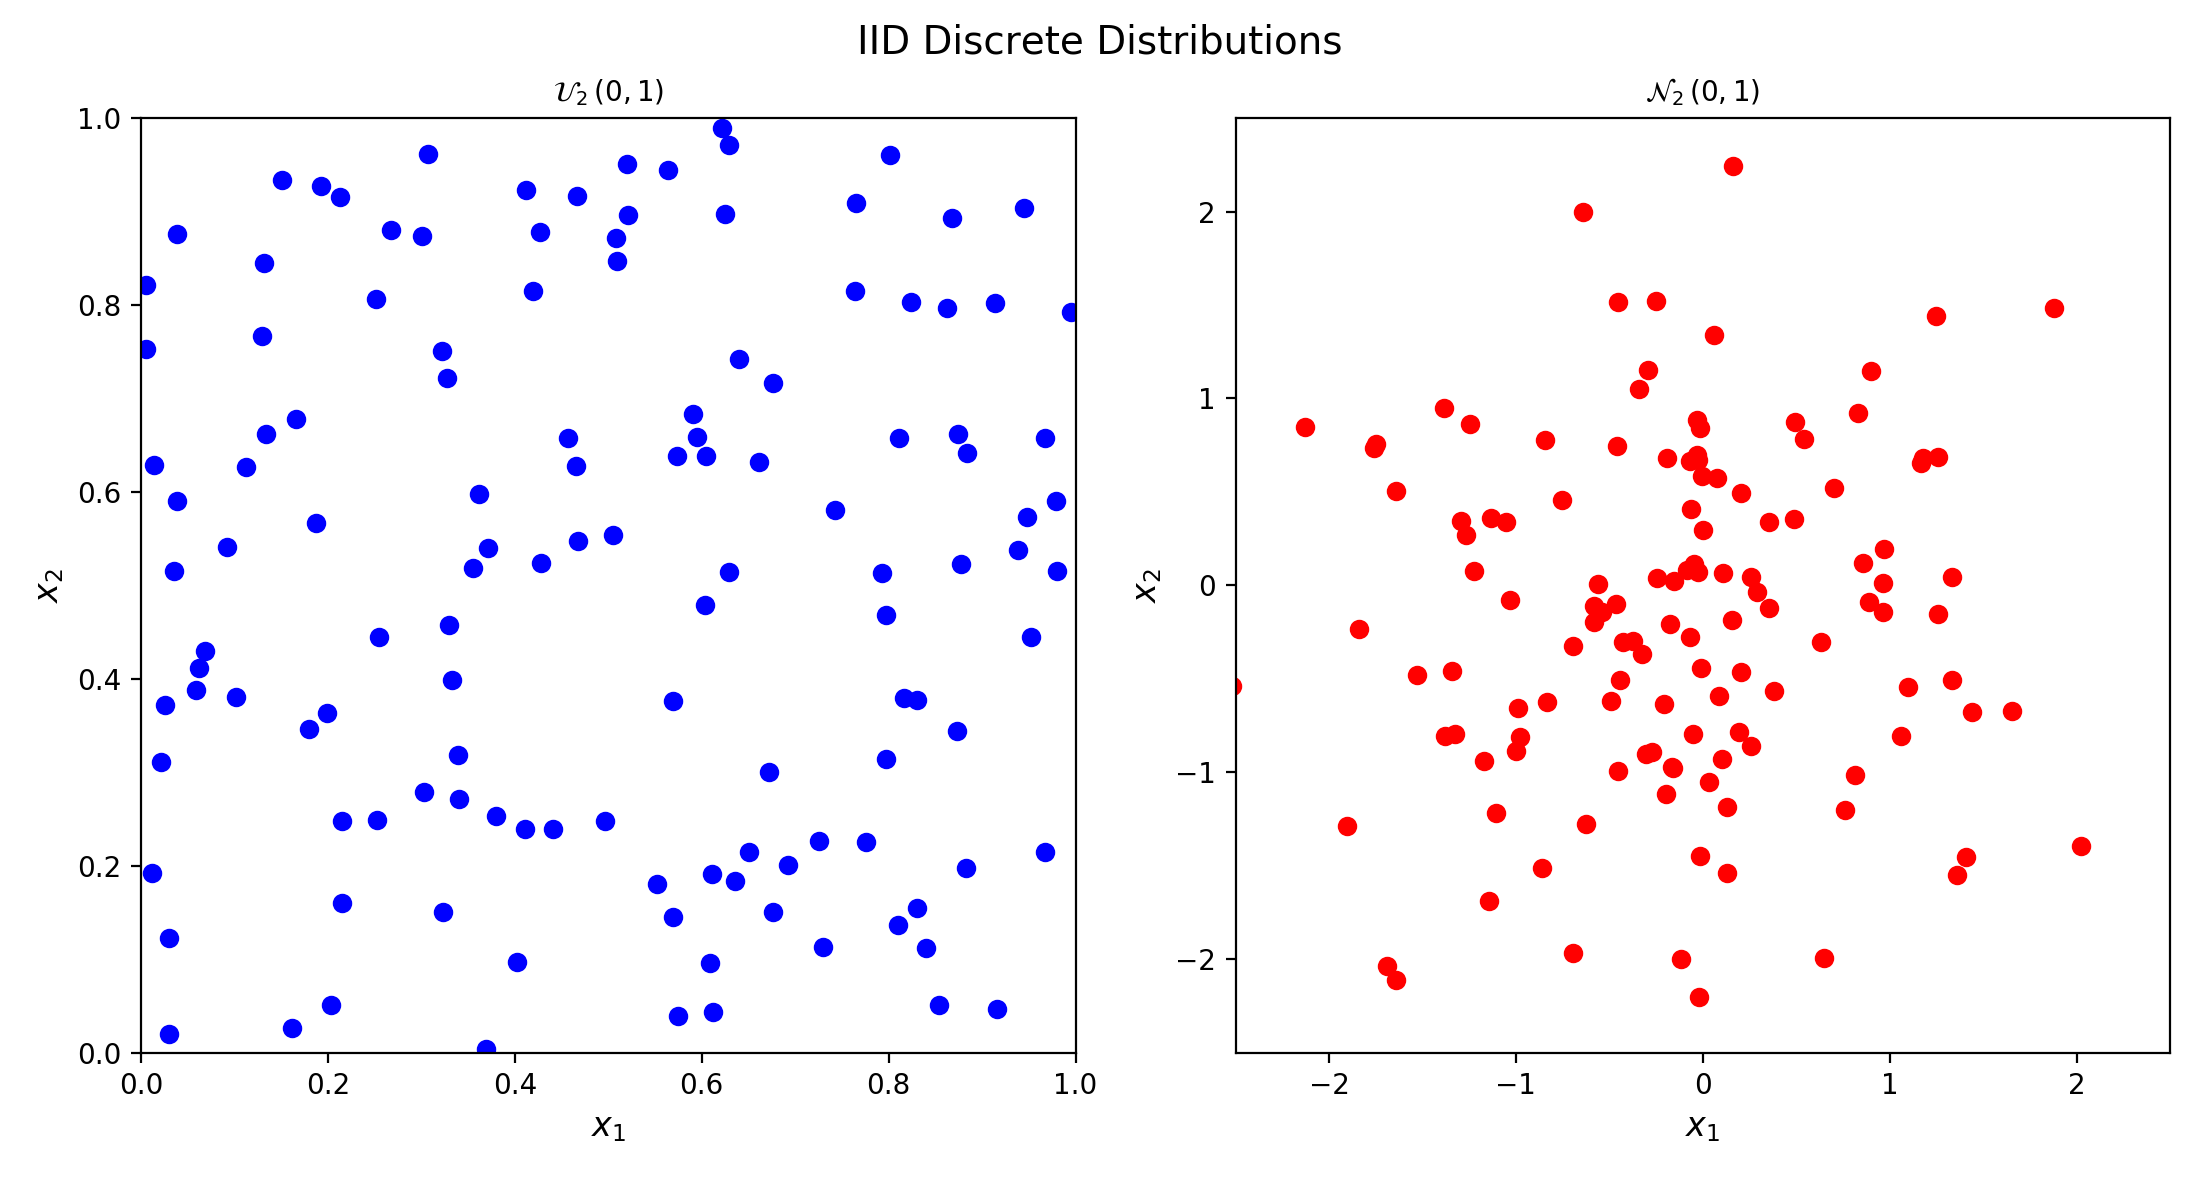
\includegraphics[width=1\textwidth]
            {Figs/iid_dd.png}
        \label{fig:iid_dd}
    \end{figure}
\end{frame}
\begin{frame}{Low Discrepancy Sequence (lds)}
    \begin{figure}[ht!]
        \centering
        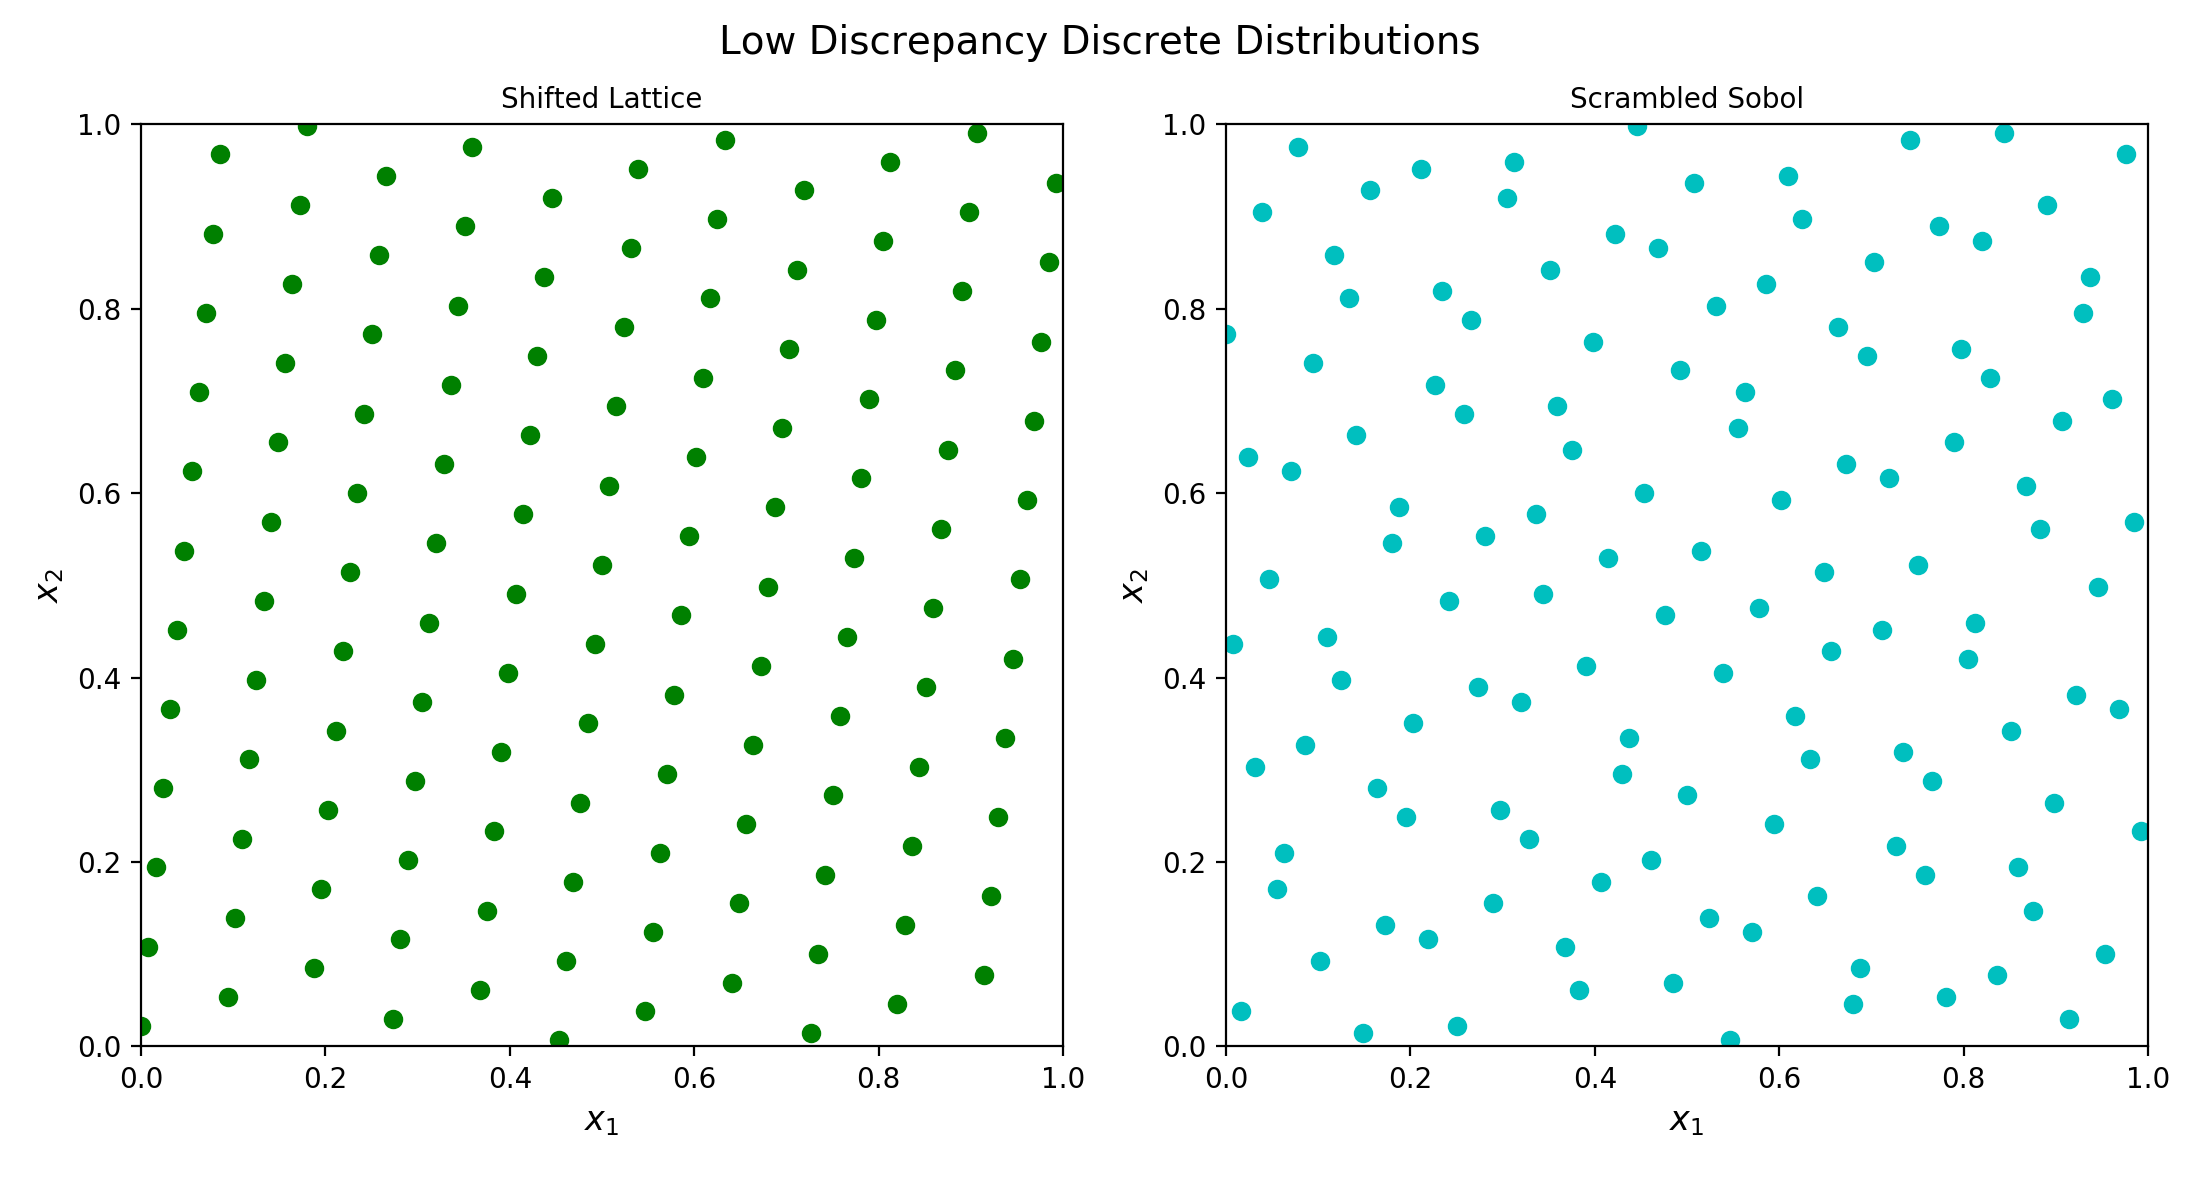
\includegraphics[width=1\textwidth]
            {Figs/lds_dd.png}
        \label{fig:lds_dd}
    \end{figure}
\end{frame}

% True Measure
\subsection{True Measure}
\begin{frame}{Uniform}
    \lstinputlisting[language=Python]{pySnips/tm.py}
    \begin{figure}[ht!]
        \centering
        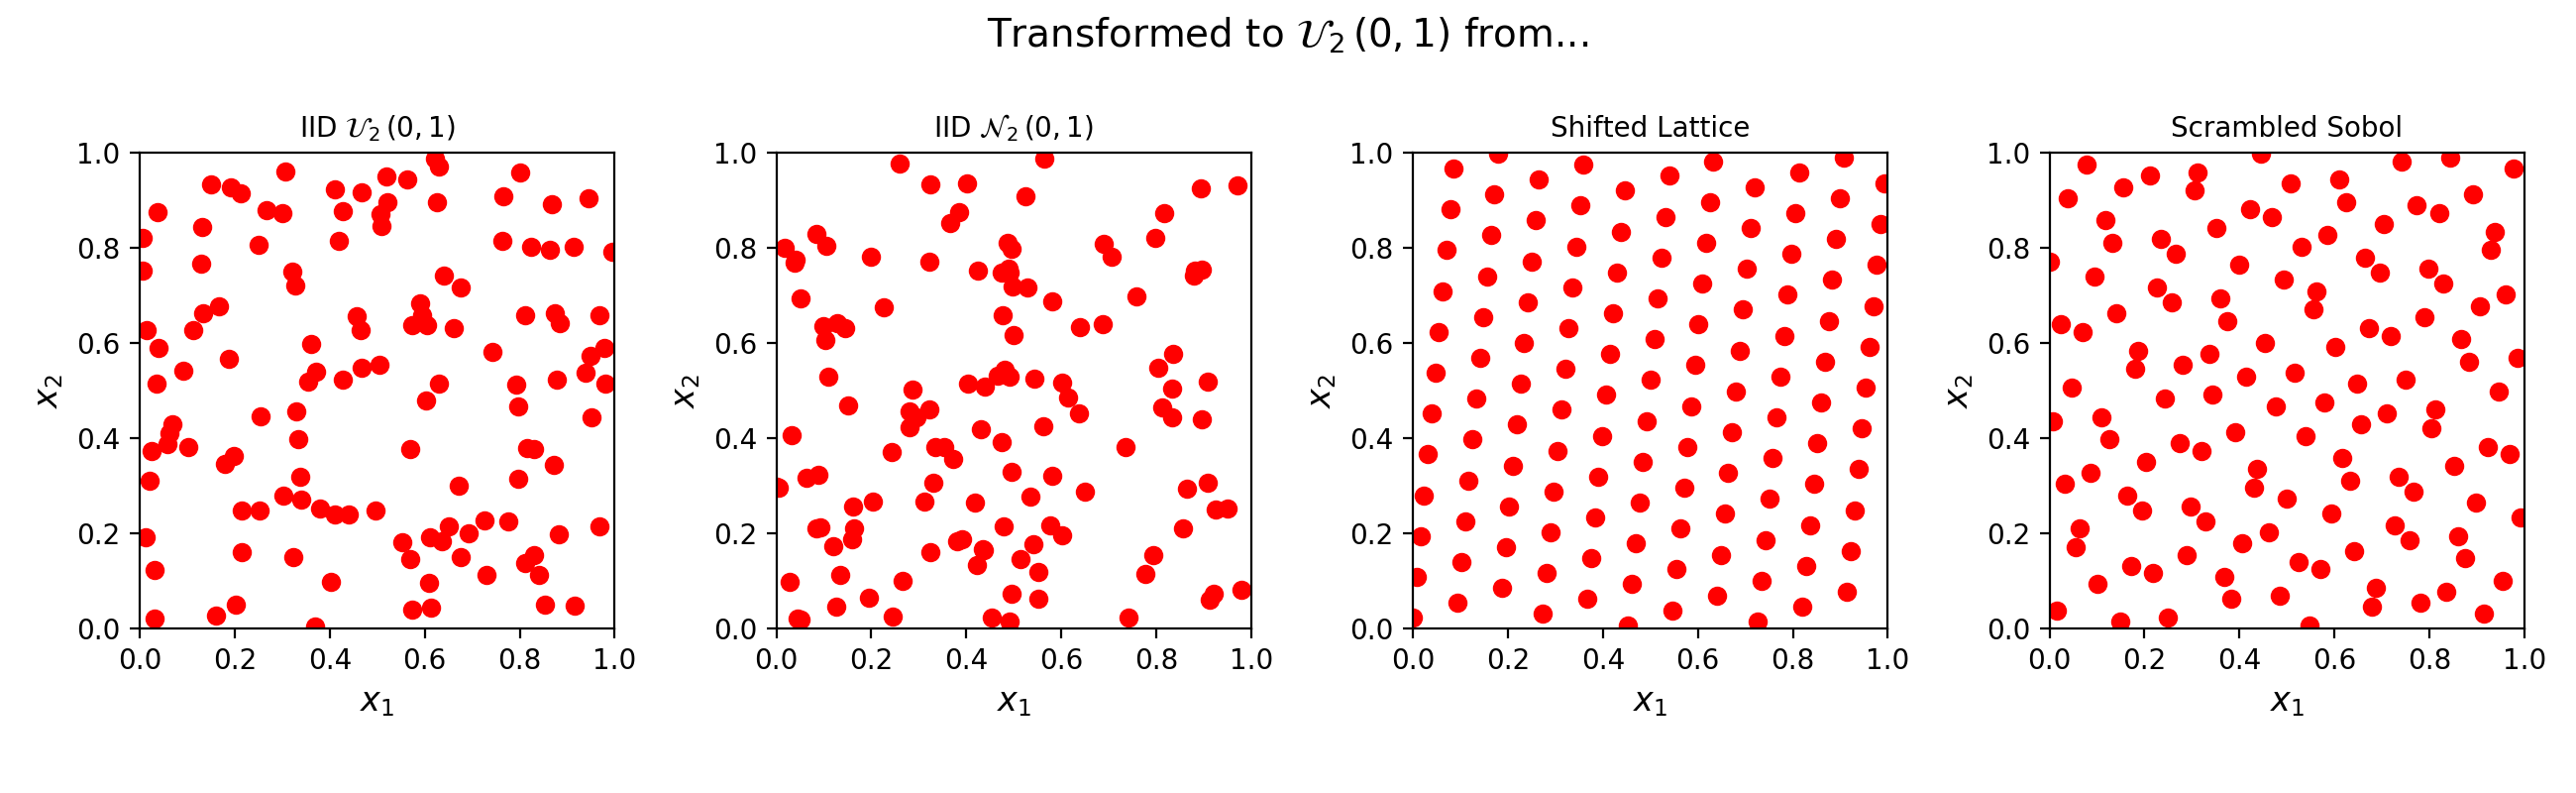
\includegraphics[width=1\textwidth]
            {Figs/Uniform_tm_transform.png}
        \label{fig:u_tm}
    \end{figure}
\end{frame}
\begin{frame}{Gaussian}
    \begin{figure}[ht!]
        \centering
        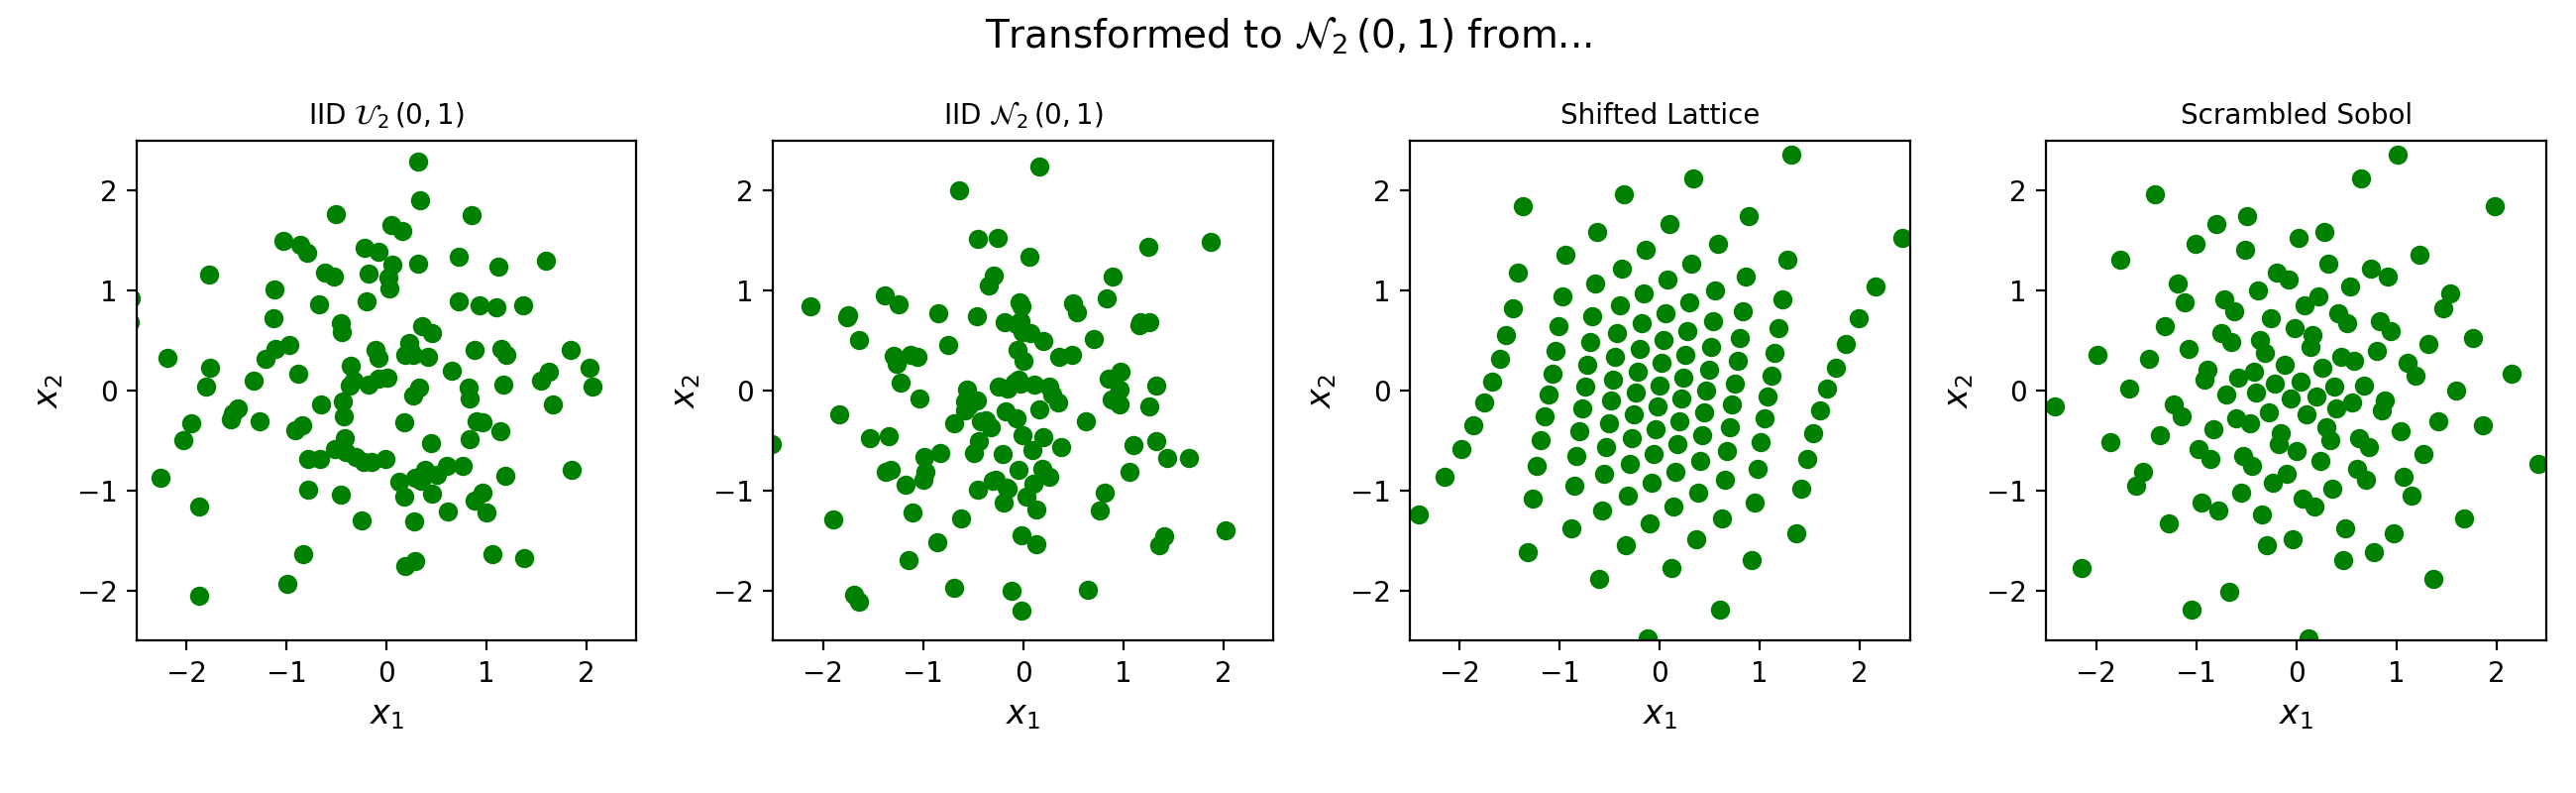
\includegraphics[width=1\textwidth]
            {Figs/Gaussian_tm_transform.png}
        \label{fig:n_tm}
    \end{figure}
    \begin{figure}[ht!]
        \centering
        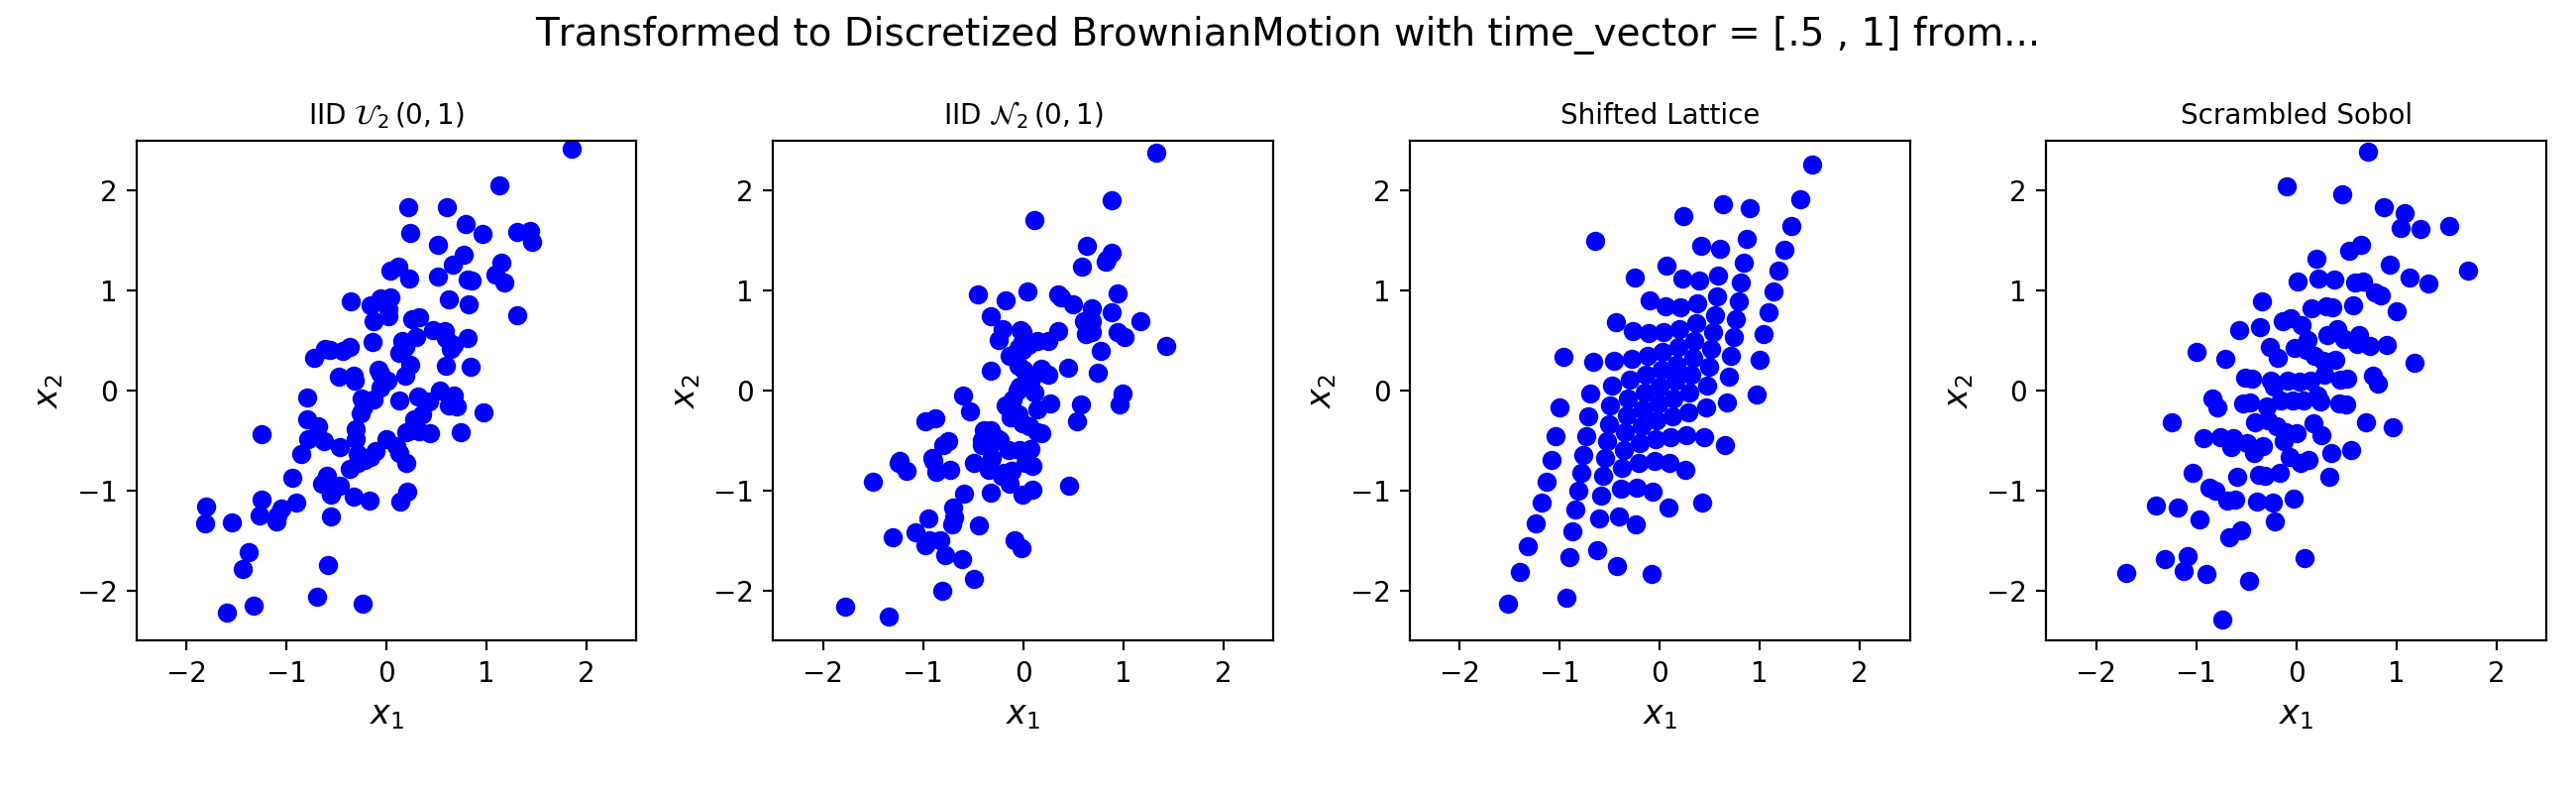
\includegraphics[width=1\textwidth]
            {Figs/BrownianMotion_tm_transform.png}
        \label{fig:bm_tm}
    \end{figure}
\end{frame}
\begin{frame}{Shift and Stretch}
    \lstinputlisting[language=Python]{pySnips/shift_stretch.py}
    \begin{figure}[ht!]
        \centering
        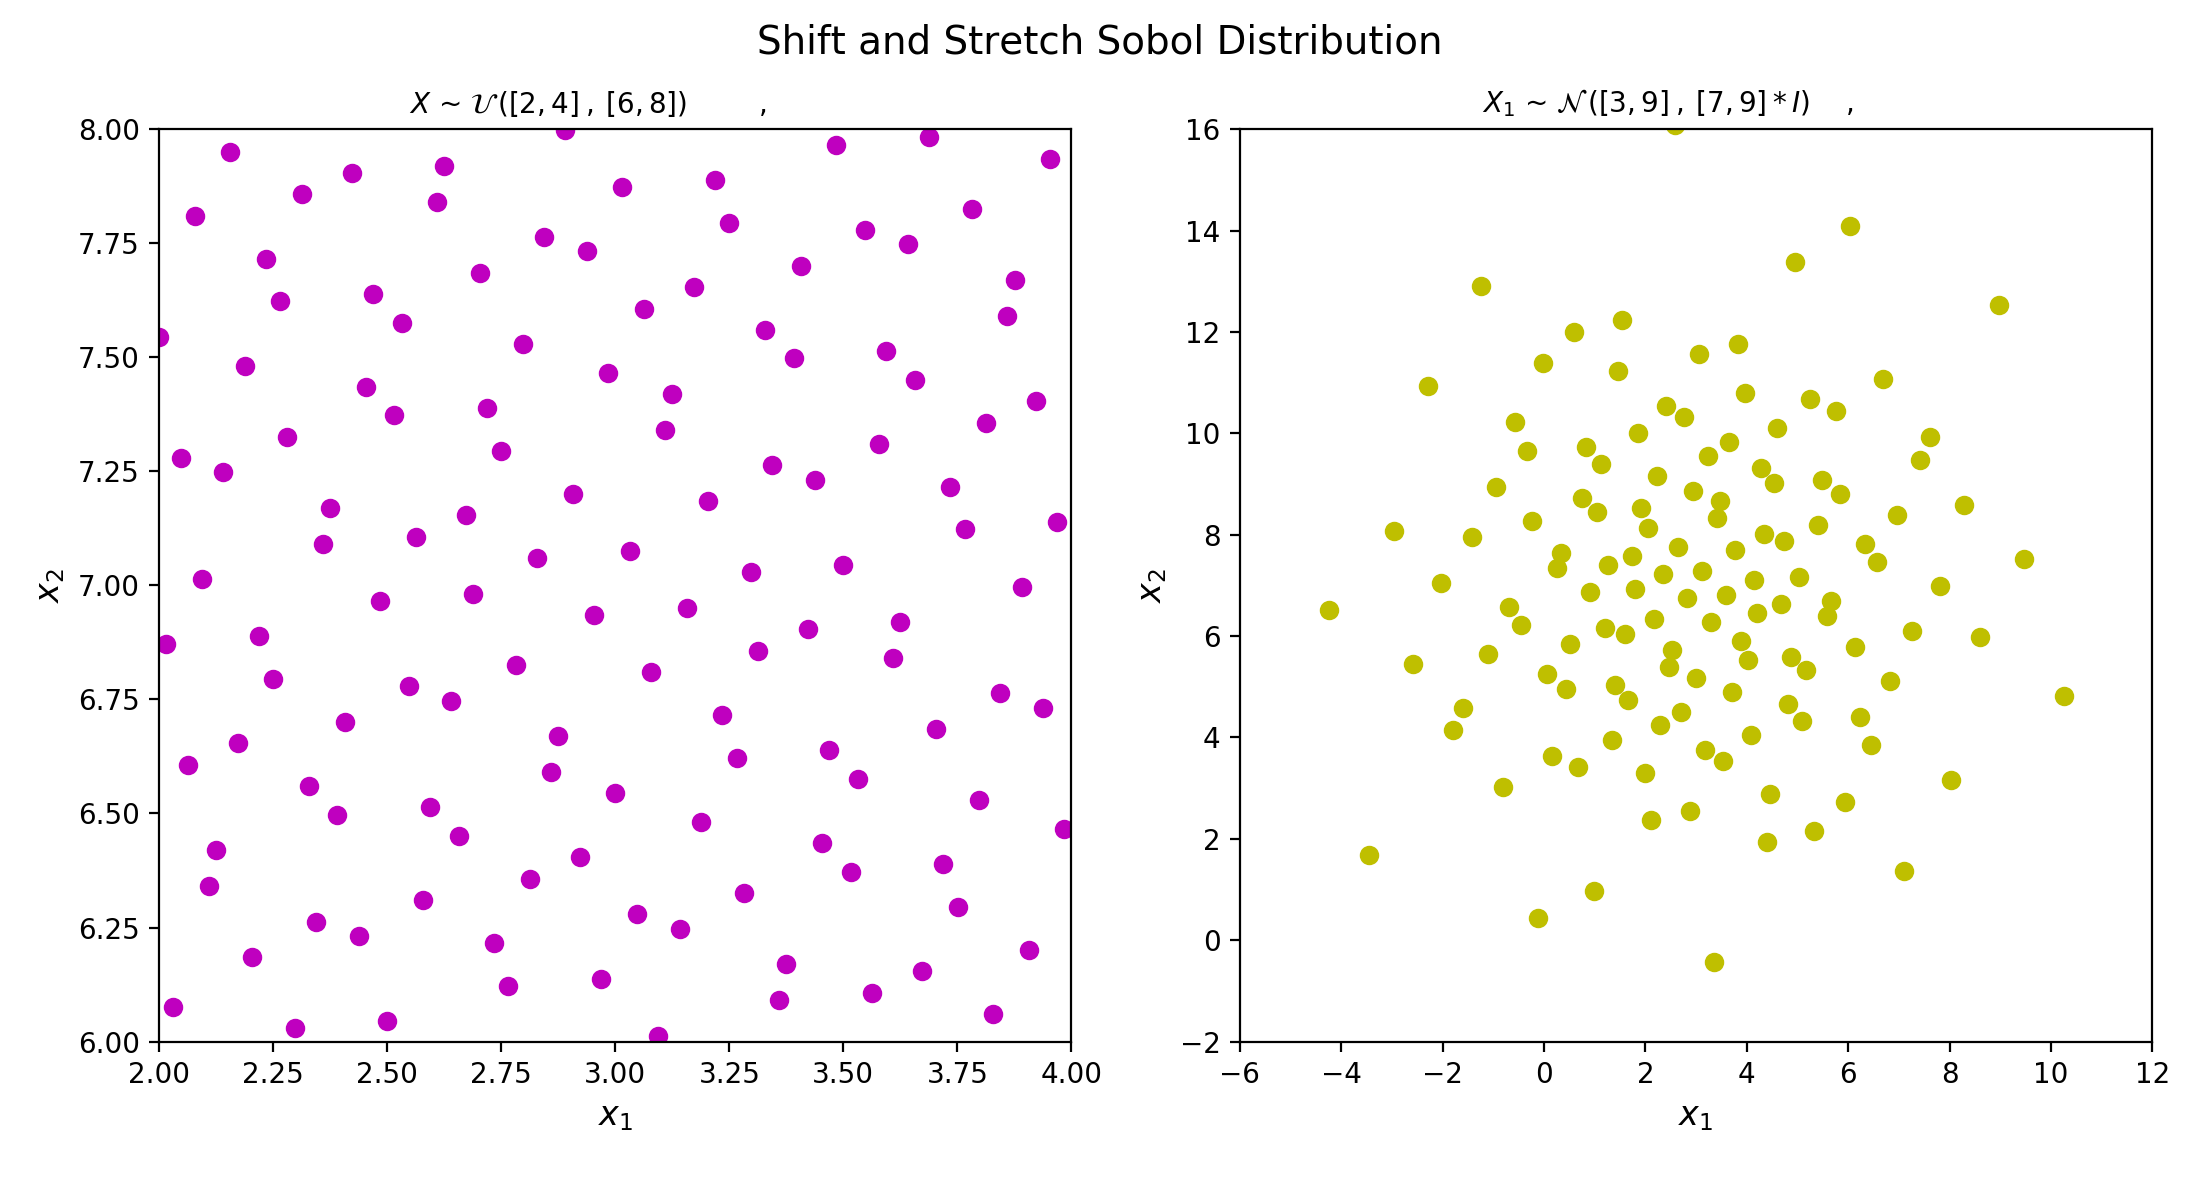
\includegraphics[width=1\textwidth]
            {Figs/shift_stretch_tm.png}
        \label{fig:ss_tm}
    \end{figure}
\end{frame}

% Stopping Criterion
\subsection{Stopping Criterion}
\begin{frame}{CLT Based Monte Carlo Algorithm for IID Nodes}
    \begin{enumerate}
        \item Choose $n_{\sigma}$ for pilot sample and compute $ \hat{\sigma}_{n_{\sigma}}^2 $
        \item For a 99\% confidence interval and inflation factor $C$, let:
            $$ n_{\mu} = \operatorname*{argmin}_n (\frac{2.58\,C\,\hat{\sigma}_{n_{\sigma}}}{\sqrt{n}} \leq \epsilon) $$
        \item Compute $ \hat{\mu}_{n_{\mu}} $ and $\hat{\epsilon} = \frac{2.58 C \hat{\sigma}_n}{\sqrt{n}}$ s.t. 
            $$ \mathbb{P}[|\mu-\hat{\mu}_{n_{\mu}}| \leq \hat{\epsilon} \leq \epsilon] \geq 99\% $$
    \end{enumerate}
\end{frame}
\begin{frame}{CLT Based Monte Carlo Algorithm for LDS Nodes}
    \begin{enumerate}
        \item Choose $n=\frac{n_0}{2}$ and number or replications $R$
        \item DO
        \begin{enumerate}
            \item $n=2n$
            \item Generate samples $\{X_j\}_{j=1}^{R}$ to compute $\{\hat{\mu}_{j,n}\}_{j=1}^{R}$ 
            \item Let $ \hat{\sigma}_n = Std(\{\hat{\mu}_{j,n}\}_{j=1}^{R})$ 
        \end{enumerate}
        WHILE $ \hat{\sigma}_n \: > \: \epsilon $
        \item Compute $\hat{\mu}_n = Mean(\{\hat{\mu}_{j,n}\}_{j=1}^{R})$ and $\hat{\epsilon} = \frac{2.58\,C\,\hat{\sigma}_n}{\sqrt{n}}$ s.t. 
            $$ \mathbb{P}[|\mu-\hat{\mu}_{n}| \leq \hat{\epsilon} \leq \epsilon] \geq 99\% $$
    \end{enumerate}
\end{frame}

% EXAMPLEs
%%%%%%%%%%%%%%%%%%%%%%%%%%%%%%%%%%%%%%%%%%
\section{Examples}
\begin{frame}{Keister Example}
    \lstinputlisting[language=Python,mathescape]{pySnips/keister_ex.py}
    \begin{figure}[ht!]
        \centering
        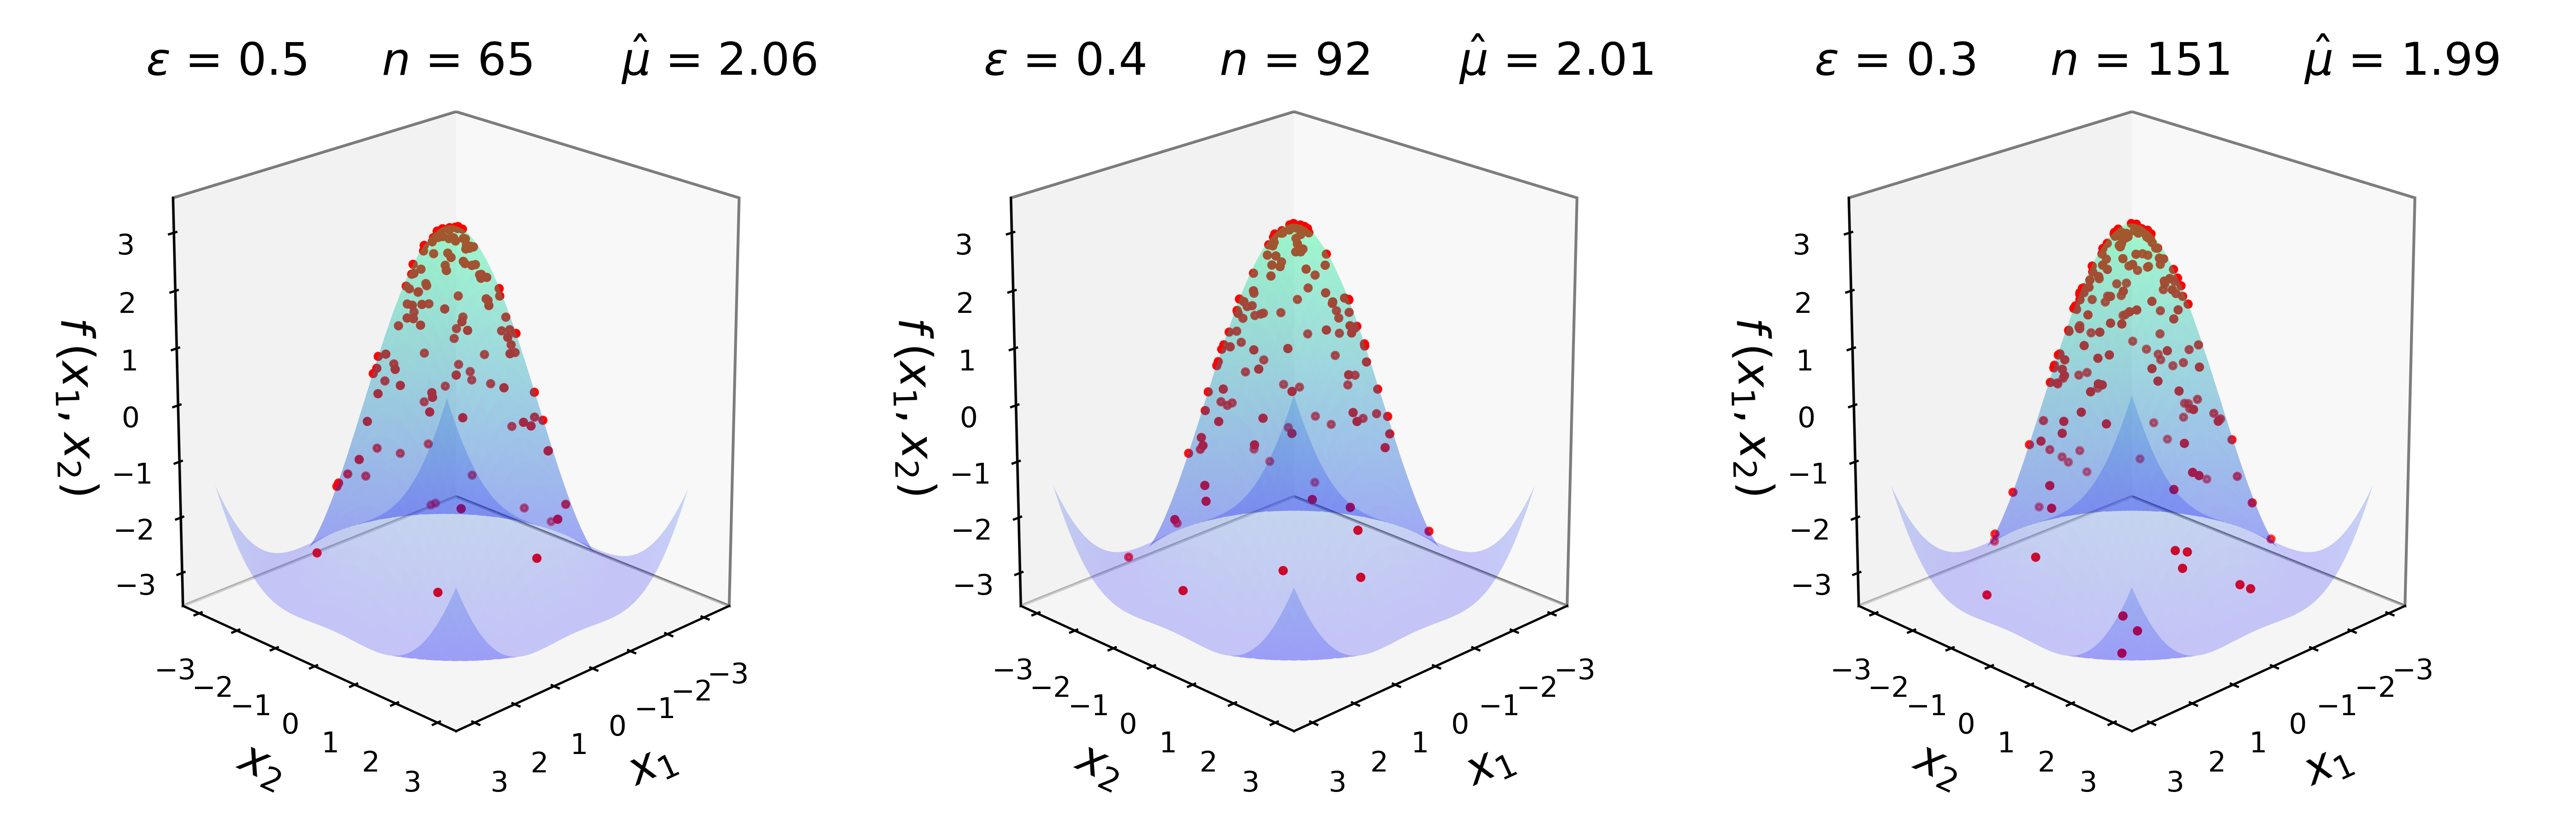
\includegraphics[width=1\textwidth]
            {Figs/Three_3d_SurfaceScatters.png}
        \label{fig:3d_keister}
    \end{figure}
\end{frame}
\begin{frame}{Keister Example Output}
     \lstinputlisting[language=Python]{pySnips/keister_ex_output.py}
\end{frame}
\begin{frame}{Multi-Level Asian Call Option Example \cite{giles2018multilevel}}
     \lstinputlisting[language=Python]{pySnips/asian_option_ex.py}
\end{frame}


% FUTURE WORK
%%%%%%%%%%%%%%%%%%%%%%%%%%%%%%%%%%%%%%%%%%
\section{Future Work}
\begin{frame}{Future Work}
    \textbf{Attract collaborators}
        \begin{itemize}
            \item i.e. Lattice, Sobol generators from Magic Point Shop \cite{mps}
        \end{itemize}
    \textbf{Expand library of components \& test cases}
        \begin{itemize}
            \item Integrand, True Measure, Discrete Distribution, Stopping Criterion
        \end{itemize}
    \textbf{Implement GAIL algorithms \cite{GAIL}}
    \begin{itemize}
        \item meanMC\_g, cubLattice\_g, cubSobol\_g \cite{mcAuto}
    \end{itemize}
\end{frame}

% Learn More
%%%%%%%%%%%%%%%%%%%%%%%%%%%%%%%%%%%%%%%%%%
\section{Project Links}
\begin{frame}{Project Links}
    \cite{qmcpy}
    \begin{itemize}
        \item \href{https://github.com/QMCSoftware/QMCSoftware.git}{GitHub}\\
            (https://github.com/QMCSoftware/QMCSoftware.git)
        \item \href{https://qmcsoftware.github.io/QMCSoftware/index.html}{Documentation}\\
            (https://qmcsoftware.github.io/QMCSoftware/index.html)
        \item \href{https://sites.google.com/hawk.iit.edu/qmc-software/home}{Website}\\
            (https://sites.google.com/hawk.iit.edu/qmc-software/home)
    \end{itemize}
\end{frame}


% REFERENCES
%%%%%%%%%%%%%%%%%%%%%%%%%%%%%%%%%%%%%%%%%%
\begin{frame}[allowframebreaks]{References}
    % 
    \bibliographystyle{amsalpha}
    \bibliography{main.bib}
\end{frame}

\end{document}
